% Results section. Numbers in the tables are generated by make_tables.py from results/*.csv.
\subsection{Forecasting, state estimation and physical consistency}
Table~\ref{tab:main} reports filtering error, open-loop forecast error at three horizons, the held-out regime, the RMS torque residual under the true parameters, and the relative error of the \SI{2}{\second} control gain. The oracle reproduces the stored trajectories exactly, which verifies the protocol. Nominal physics shows how much the hidden parameters matter: with catalogue parameters it is far worse than any learned model.

The two-stage JEPA world model, read out by a frozen probe fitted on 300 labelled episodes, roughly halves the reconstruction world model's \SI{2}{\second} error with a linear probe, and is still clearly better with an MLP probe. The pipeline given the true ODE form remains the most accurate in distribution. Full supervision with 3000 labels lies between the two (Fig.~\ref{fig:horizon}).

\begin{table*}[!t]\centering\scriptsize
\caption{Main results, mean $\pm$ s.d. over seeds. Rotor-speed RMSE in \si{\radian\per\second}. Torque residual in \si{\newton\metre}. Gain error is the median relative error of $\partial\hat\omega(t_0+\SI{2}{\second})/\partial u$.}
\label{tab:main}
\tablefile{main}
\end{table*}

\begin{figure}[!t]\centering
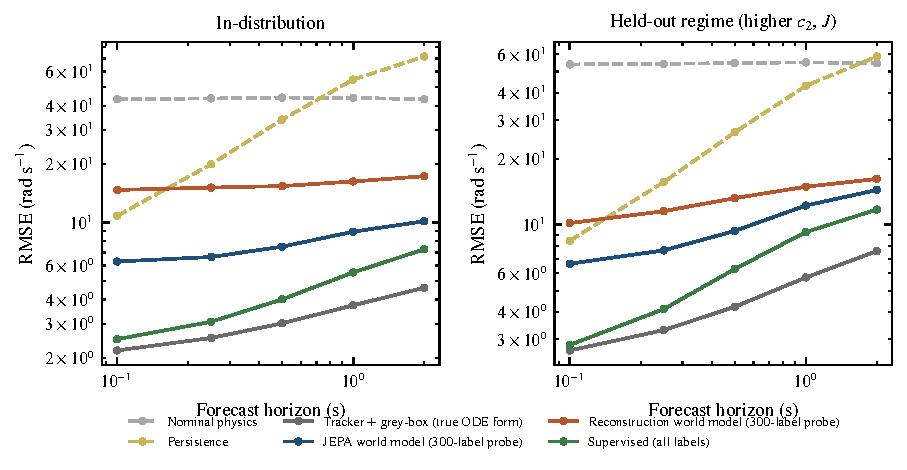
\includegraphics[width=\columnwidth]{fig_horizon.pdf}
\caption{Forecast error against horizon, in distribution (left) and in the held-out regime (right). Bands span seeds.}
\label{fig:horizon}
\end{figure}

\subsection{Label efficiency}
Fig.~\ref{fig:labels} and Table~\ref{tab:labels} show the result that matters most for a test cell, where unlabelled acoustic logs are cheap and tachometer-labelled runs are not. At every budget up to 300 labelled episodes, a JEPA world model, either frozen with a linear probe or fine-tuned, forecasts better than the same network trained from scratch on the same labels. The gap is largest at 10--30 episodes.

\begin{figure}[!t]\centering
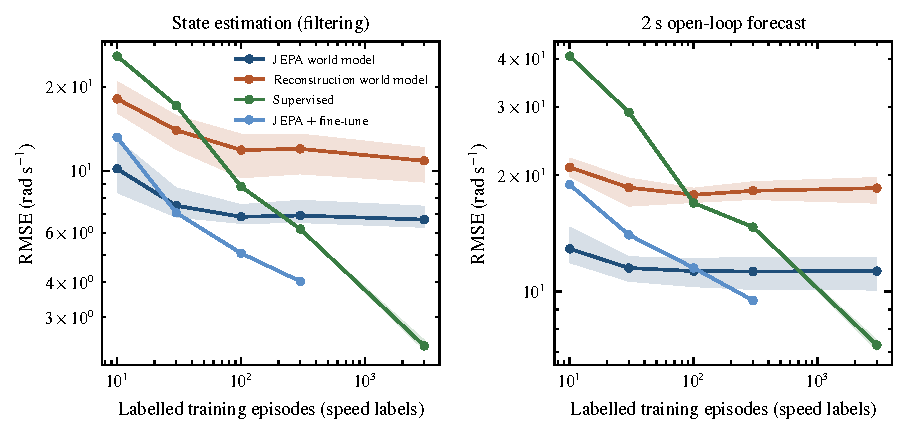
\includegraphics[width=\columnwidth]{fig_label_efficiency.pdf}
\caption{Filtering and \SI{2}{\second} forecast error against the number of speed-labelled training episodes. Every self-supervised model also sees all 3000 unlabelled episodes.}
\label{fig:labels}
\end{figure}

\begin{table}[!t]\centering\scriptsize
\caption{\SI{2}{\second} forecast RMSE (\si{\radian\per\second}) against labelled episodes.}
\label{tab:labels}
\tablefile{labels_forecast}
\end{table}

\subsection{Robustness to nuisance}
The harmonic tracker that feeds the classical pipeline locks onto distractor tones once they are frequent (Fig.~\ref{fig:nuisance}, $\lambda\geq2$), and its forecast error grows several-fold by $\lambda=3$. The learned belief degrades smoothly. By $\lambda=3$ the JEPA world model and the supervised model both forecast better than the structure-aware pipeline, although they were trained only at $\lambda=1$. Table~\ref{tab:nuisance} also reports models trained at $\lambda=2.5$.

\begin{figure}[!t]\centering
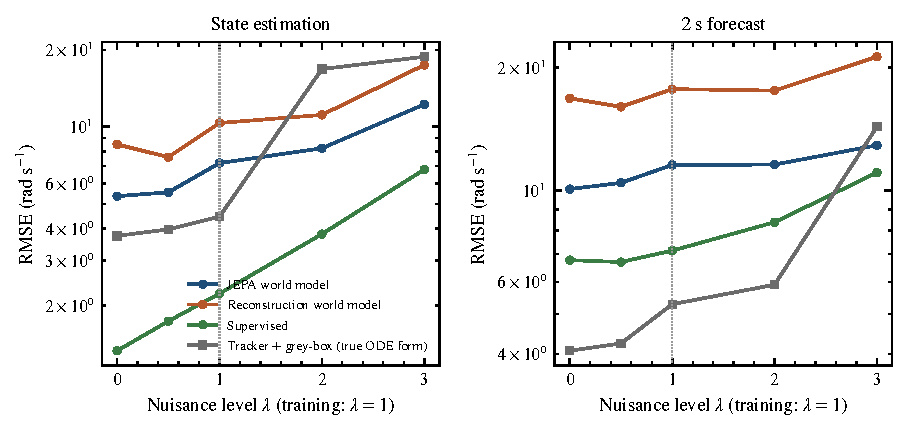
\includegraphics[width=\columnwidth]{fig_nuisance.pdf}
\caption{Filtering and forecast error against test nuisance level $\lambda$; learned models trained at $\lambda=1$.}
\label{fig:nuisance}
\end{figure}

\begin{table}[!t]\centering\scriptsize
\caption{\SI{2}{\second} forecast RMSE against test nuisance $\lambda$.}
\label{tab:nuisance}
\tablefile{nuisance_forecast}
\end{table}

\subsection{Control authority and hidden parameters}
Every learned model now reproduces the plant's step response to a command change (Fig.~\ref{fig:step}), the property whose absence was the main v1 failure. This follows from training on time-varying commands rather than from any architectural trick. Linear probes on the latent at $t=\SI{2}{\second}$ (Table~\ref{tab:probes}) recover the steady-state gain ($k_\omega$) well and the actuator lag partly. They recover essentially nothing of the inertia, mass flow or transport delay. The latent captures \emph{state} better than it \emph{identifies the machine}, and this is the main reason the true-structure grey-box still wins on long in-distribution forecasts.

\begin{figure}[!t]\centering
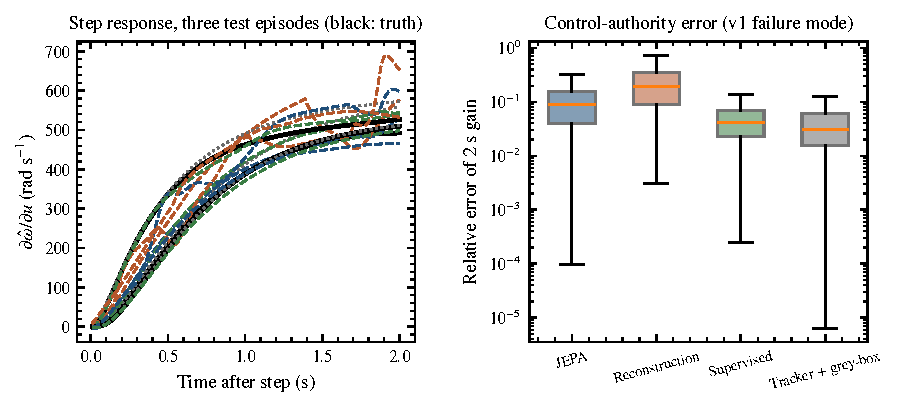
\includegraphics[width=\columnwidth]{fig_step_response.pdf}
\caption{Left: model step responses (dashed) against simulator finite differences (black) for three test episodes. Right: relative error of the \SI{2}{\second} gain over the test set.}
\label{fig:step}
\end{figure}

\begin{table}[!t]\centering\scriptsize
\caption{Linear-probe $R^2$ for hidden parameters from $z_{t=\SI{2}{\second}}$ (300 labelled episodes).}
\label{tab:probes}
\resizebox{\columnwidth}{!}{\tablefile{param_probes}}
\end{table}

\subsection{Closed-loop control by planning in latent space}
Table~\ref{tab:mpc} and Fig.~\ref{fig:mpc} compare CEM-MPC controllers that differ only in their model, tracking moderate set-point steps from the spectrogram alone. We report excess tracking MSE over an oracle controller with the true parameters and state, with paired bootstrap intervals. Planning through the JEPA latent comes close to the oracle and to the true-structure grey-box. With the same 300 labels, JEPA pre-training reduces excess error several-fold relative to supervised training from scratch, and the gap widens at $\lambda=3$. A PI controller on the tracked speed is far worse, and it fails when the tracker fails.

\begin{figure*}[!t]\centering
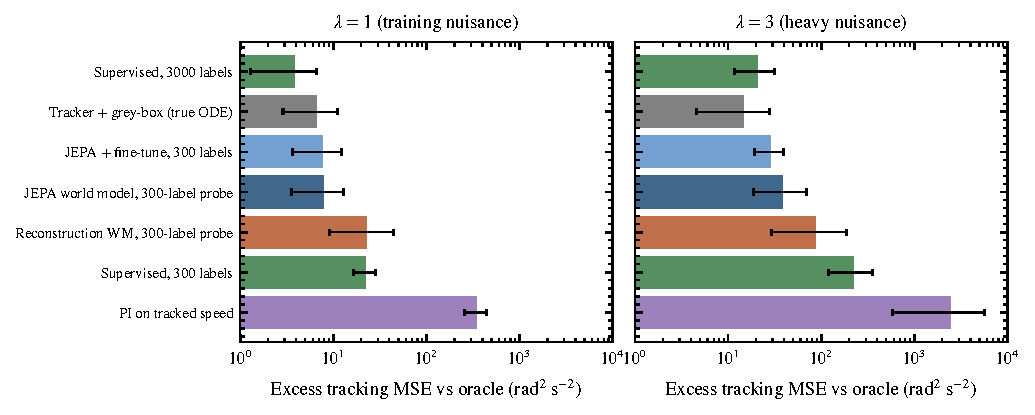
\includegraphics[width=0.78\textwidth]{fig_mpc.pdf}
\caption{Closed-loop excess tracking MSE over the oracle (40 test episodes, paired bootstrap 95\% CIs) at the training nuisance (left) and heavy nuisance (right).}
\label{fig:mpc}
\end{figure*}

\begin{table}[!t]\centering\scriptsize
\caption{Closed-loop tracking at $\lambda=1$ (seed-0 models).}
\label{tab:mpc}
\resizebox{\columnwidth}{!}{\tablefile{mpc}}
\end{table}

\subsection{Ablations}
Table~\ref{tab:ablations} isolates the design choices on seed 0. Long-horizon training (\SI{1.28}{\second} rollouts on \SI{3.2}{\second} crops) gives the largest single gain, and it helps every objective, not only JEPA. Removing stage-1 pre-training, by freezing a random trunk, hurts both perception and forecasting. An explicit adaptive context embedding made forecasts worse; we report it as a negative result.

\begin{table*}[!t]\centering\scriptsize
\caption{Seed-0 ablations (300-label linear probe where applicable).}
\label{tab:ablations}
\tablefile{ablations}
\end{table*}
